%\setcounter{chapter}{4}
\chapter{ Appendix Chapter 4: Application of general matching}

\section{Two processor scheduling}\index{Two processor scheduling}

Given:\\
\begin{enumerate}
  \item Two identical agents/processors
  \item Collection of n jobs or tasks together with a directed acyclic graph with n nodes which correspond to the jobs, that describe the preceedence among the jobs.
\end{enumerate}


\begin{example}
\begin{figure}[h]
\centering
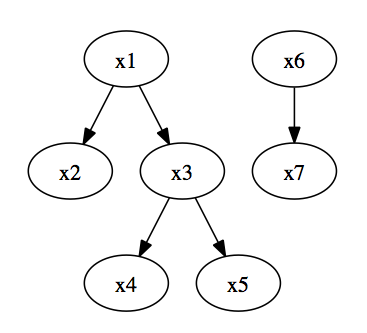
\includegraphics[scale=0.4]{diagrams/gapp4.png}
\caption{Graph G}
\end{figure}

\begin{figure}[h]
\centering
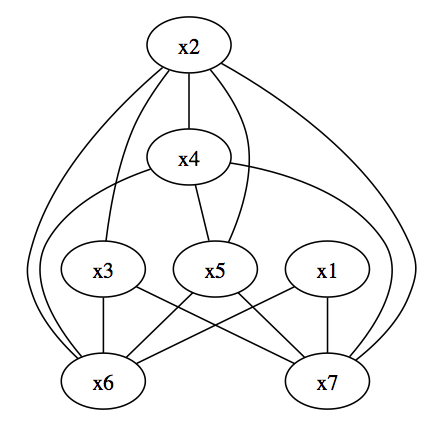
\includegraphics[scale=0.4]{diagrams/g2app4.png}
\caption{Graph G*}
\end{figure}
\end{example}

How can the jobs be scheduled on the two processors such that the jobs are completed as quickly as possible?

\textbf{Solution}:\\
using matching!\\
\underline{But:}\\
for three processors the problem is NP-Complete.\\

To solve the two processors problem we proceed as follows. We construct a graph $G*$ that has the same nodes as $G$ and there is an edge {x,y} in $G*$ if and only if there is no path from x to y in $G$ and no path from y to x in $G$.

\underline{1. Observation:}\\
if we have a schedule we can obtain a matching. If the schedule is optimal the matching is of maximal cardinality.

\underline{2. Interessting:}\\
We can use matching of maximal cardinality to produce a schedule that is optimal.\\

Let S be a set of nodes with indegree 0. Let $M*$ be a matching of max. cardinality for $G*$. Apply the following rules repeatly:\\
\begin{enumerate}
  \item If there is an unmatched node in S then schedule it. Remove it from G.
  \item If there is a pair of nodes (jobs) in S that is matched in $M*$ then we schedule this pair and delete the two nodes (corresponding to the jobs) in G (i.e. that an edge in $M*$ starts/ends at the nodes of the pair).
\end{enumerate}


<<<< Start MS - Description\\
If neither rule 1 nor rule 2 applies and there are still jobs left to be scheduled then we know that S contains only nodes that are matched
and for every node in S its partner ($M*$) is not in S.\\

$J{_1} \in S$ ------$M*$------
$J'{_1} \notin S$\\

$J{_2} \in S$ ------$M*$------
$J'{_2} \notin S$\\

Observation:\\
$\not\exists$ path $J_{1}$ to $J_{2}$ \\
<<<< End MS - Description

<<<< Start NW - Description \\
 If none of the above rules is applicable anymore we know that S contains only nodes that are matched, otherwise rule 1 would be applicable.\\
 Moreover each job in S is matched to a job not in S, otherwise we could schedule the matched pair. \\
  $ J_{2} \not\in S$ --- $ e\in M*$ --- $J_{2}' \in S \rightarrow J_{1}' \not\in S$  --- $ e\in M*$ --- $ J_{1} \in S$ \\
 To continue the scheduling we consider the following:\\
 Observation i):\\
 There is no path from $J_{1}'$ to $J_{2}'$ because otherwise ther could be the path $J_{2} \rightarrow J_{1}' \rightarrow J_{2}'$ and $J_{2},J_{2}'$ could not be matched in $M*$.\\
 \newline
 Observation ii):\\
 There is no path from $J_{1}$ to $J_{2}$ for the same reason. \\
 \newline
 Observation iii): \\
 There is no path from $J_{2}$ to $J_{1}$ because $indegree(J_{1})=0$ and there are no cycles in G.\\
 \newline
 Observation iv): \\
 case1: If there is no path from $J_{2}'$ to $J_{1}'$, then we can subsitute in $M*$ the pairs $\{ J_{2}, J_{2}' \}$ and  $\{ J_{1}, J_{1}' \}$ by $\{ J_{1}, J_{2'} \}$ and $\{ J_{1}', J_{2} \}$ in $G*$. Now $\{ J_{1}, J_{2}' \}$ is $\in M*$ and can be scheduled according to rule ii). \\
 case2: If there is a path from $J_{2}'$ to $J_{1}'$ we repeat the same argumentation as before. \\
 \newline
 The process terminates, because the graph G is finite and cycle free.
 
<<<< End NW - Description \\



